\section{Modeling for Constraint Solver}
\label{impl:solver}

As explained in previous chapters, our framework employs a general solver for constraint
satisfaction problems (CSPs). We have chosen Choco solver~\citep{choco}, a free and
open-source constraint programming library for Java. Much of the work the framework does
is converting the ensemble configuration into a problem input for Choco solver. This
section explains the process in detail.

%%%

\subsection{Overview of Choco Solver}

Choco is a very fast constraint solver, designed with research applications in mind. It
is written in Java 8, which allows us to integrate it easily with our Scala framework.
Out of the box, Choco supports integer, boolean, and real values, and sets of integers.
It allows the users to constrain domains of variables with basic equalities and
inequalities, simple arithmetic expressions, boolean operations, automatons,
if/then/else expressions, membership conditions, etc. It is also possible to implement
custom constraints and their propagators.

Choco's key component is a \cc{Model} object, which represents the problem currently
being solved. Methods of this objects can be used to create \textit{variables} of
different types. For our framework, we make use of \cc{BoolVar}, \cc{IntVar} and
\cc{SetVar}.

\medskip

Domain of a \cc{IntVar} is $[-2^{32}, 2^{32}-1]$. It can be represented in two distinct
ways: a \textit{bounded} domain is a contiguous interval between the upper and lower
bound, while an \textit{enumerated} domain can be any set of integers. The latter is
obviously less performant and memory-efficient. However, for our use-case, we only use
enumerated domains.

Domain of a \cc{BoolVar} is $\{0, 1\}$, i.e., it is implemented as an integer. The
important feature of \cc{BoolVar} is that it can be used for \textit{reification} of
constraints; i.e., the resulting value of the variable represents whether a particular
constraint was satisfied or not.

Domain of a \cc{SetVar} is any set of integers. The default internal representation is a
bit set, through Java's \cc{BitSet} data type. We use set variables to represent
ensemble or role membership. Integers in the set represent indices into an array that
holds the member objects.

\medskip

Each constraint is also represented as a Java object, generated by a factory method on
the \cc{Model} instance. Every constraint can either be \textit{posted} or
\textit{reified}.

Posting a constraint means that it will represent a rule in the model. Every solution
\textit{must} satisfy that constraint.

Reifying a constraint associates it with a boolean variable. That variable resolves to
true if the constraint is satisfied, or false if not. This allows expressing constraints
as boolean expressions or if-then constructs based on the status of other constraints.

Choco solver provides a rich library of built-in constraint constructors. Arbitrary
arithmetic operations on \cc{IntVar}s are available, as well as tests of set
membership, intersections, union, subset relation, etc. More complex constructions can
be built with boolean operators, and it is possible to set up constraint dependencies
with \cc{ifThen} and \cc{ifOnlyIf} methods.

%%%

\subsection{Modeling Basics}

At its heart, ensemble assignment is a set membership problem. It makes sense that the
basic building block would be a \cc{SetVar}. The framework assembles components and
ensembles into \textit{groups}, and each group is represented by a \cc{SetVar} over the
entities' indices within the group: if an index is included in the \cc{SetVar}, the
corresponding entity is considered part of the solution, and we say it is
\textit{selected}.

Per-group sets mean that the same entity can have a different index in different groups.
That makes certain operations awkward. Namely, in many cases we cannot use the built-in
set operations, because for a given index $n$, $n \in A$ usually represents a different
entity than the same $n \in B$. This makes operations like set union meaningless and we
need to reconstruct them from primitives.

The alternative would be to assign an unique index to every entity and represent
membership through these unique indices. However, that would lead to sparse sets, which
would make their in-memory representations inefficient.

In case of ensembles, there is an implicit dependency relationship: a child ensemble can
be selected if and only if its parent is also selected. Similarly, if an ensemble is not
selected, no components are selected for any of its roles. These dependencies must be
expressed as constraints on group membership.

%%%

\subsection{Ensemble Selection and Situations}

Several things must be true if an ensemble is selected: its parent must also be
selected, its situation predicate must not be false, and all of its constraints must be
satisfied. These requirements can be expressed in simple implications:

\begin{enumerate}
\item Root ensemble is always selected.
\item \textbf{IF} parent ensemble is not selected, \textbf{THEN} none of its children
    are selected.
\item \textbf{IF} ensemble is selected, \textbf{THEN} its situation predicate must be
    true, and its constraints must be satisfied.
\end{enumerate}

No rule specifies when an ensemble \textit{should} be selected, though. With the
exception of the root ensemble, this means that the simplest solution is to not select
any ensembles.

There are steps the user can take to avoid this problem. They can specify constraints in
the root ensemble that enforce existence of some or all sub-ensembles, or they can
configure utility functions in a way that maximizes the number of selected ensembles,
etc. The drawback of these approaches is their obscurity. The problem itself is
non-obvious, why should the policy designer think about resolving it in the first place?

Furthermore, the natural way of writing ensemble selection constraints is indirect,
through the ensemble's properties or membership of its roles. But in such case, the
variable representing ensemble selection remains free. This is a performance hit, in the
form of larger search space: the solver will still attempt to find solutions that
satisfy the constraint with various configurations of selected ensembles. Using an
utility function is similar: even though a solution with more ensembles is better, other
solutions are not \textit{invalid} and might still need to be examined.

In some cases, this behavior is desirable. In access control scenarios, however, it is
rarely needed. Most cases can be solved by keying ensemble selection either to the
resource being accessed, or to privileged actors --- even if the corresponding set of
actors or subjects ends up being empty.

To facilitate that, ensembles registered via the \cc{rules} call have mandatory
selection based on the situation predicate. The following rule is added:

\begin{enumerate}
\setcounter{enumi}{3}
\item \textbf{IF} parent ensemble is selected, \textbf{AND} child's situation predicate
is true, \textbf{THEN} child ensemble is also selected.
\end{enumerate}

Using (1) together with (4), it is easy to derive membership status of every ensemble
registered with \cc{rules}.

%%%

\subsection{Constraint Propagation}
\label{impl:solver:constraints}

To make use of Choco solver's constraint programming machinery, all constraints must be
posted as instances of the \cc{Constraint} class. To do otherwise would be highly
inefficient; the solver would present us with an exhaustive list of solutions,
exponential in the number of elements, and the framework would check constraint
applicability on each one. This is the work we are trying to avoid by using a CSP solver
in the first place.

As designers of the DSL, we want to allow the user to write constraint expressions with
the language's operators. If we were designing an external DSL with custom parsing, we
could convert the expressions to solver concepts. In an internal DSL, however, there is
already a well-defined syntax and semantics for integer and boolean operations.

There are two kinds of constraints. Logical constraints place requirements on truth
values of statements: a particular component is or is not a member of a particular role;
a predicate holds for all or some members of the role, and similar. Arithmetic
constraints place requirements on results of calculations and establish equalities or
inequalities between integer values. Of course, an arithmetic constraint still boils
down to a truth value of a statement. However, calculations with \cc{Int}s in the host
language must be properly converted to Choco's \cc{IntVar}s and the arithmetic
predicates on them.

%%%

\subsection{Logical Constraints}

Logical constraints are represented by the trait \cc{Logical}, which emulates the
built-in \cc{Boolean} type. The trait defines the following operators: \dop{&&}
(conjunction), \dop{||} (disjunction), \dop{->} (implication), \dop{<->} (equivalence),
and unary \dop{!} (negation). Implication is defined in terms of disjunction and
negation, and equivalence is defined as an implication in both directions. The remaining
operators must be defined in implementations of \cc{Logical}.

There are three concrete implementations: \cc{LogicalBoolean}, \cc{LogicalBoolVar} and
\cc{LogicalLogOp}.

\medskip

\cc{LogicalBoolean} simply boxes the native \cc{Boolean} type in a \cc{Logical}
interface. Any time a \cc{Boolean} value comes into contact with a \cc{Logical}, it is
implicitly converted to \cc{LogicalBoolean}. This allows us to define all operators with
\cc{Logical} operands.

Having a constraint type whose value is statically known is also useful for
short-circuiting. A complicated boolean expression needs to be converted to Choco
constraints if the values of variables are unavailable, but can be evaluated directly
when they are known. The framework makes use of short-circuiting in several places; most
notably, when generating a list of constraints for an ensemble. All ensemble constraints
must be satisfied, so if a \cc{LogicalBoolean(false)} is found, the whole set of
constraints evaluates to false.

\medskip

\cc{LogicalBoolVar} is backed by Choco's \cc{BoolVar}, and \cc{LogicalLogOp} is backed
by a \cc{LogOp}. The difference is a matter of Choco implementation: \cc{BoolVar}
represents a \textit{variable} in the constraint problem, while a \cc{LogOp} represents
a \textit{constraint}, namely, a tree of boolean clauses in Choco's SAT constraint
propagator. Both share a common interface \cc{ILogic}. The framework defines a common
superclass \cc{LogicalWithILogic}, which implements the ``\cc{&&}'' and ``\cc{||}''
operators. Short-circuiting is used here too: if one of the operands is a
\cc{LogicalBoolean}, the result is either a fixed truth value or the value of the other
operand. Only when both operands are \cc{LogicalWithILogic}s, a new \cc{LogOp} is
created.

The only difference between a \cc{BoolVar} and a \cc{LogOp} is negation. A \cc{BoolVar}
class has a \cc{not()} method; for \cc{LogOp}, no such method is available and the
negation must be constructed from a \cc{nand} operation.

%%%

\subsection{Arithmetic Constraints}
\label{impl:solver:arithm}

Arithmetic constraints are represented by the trait \cc{Integer}, which emulates the
built-in \cc{Int} type. The trait defines the basic arithmetic operators \dop{+},
\dop{-} (including unary minus), \dop{*}, and \dop{/}; and comparison operators
\dop{===}, \dop{!=}, \dop{<}, \dop{>}, \dop{<=}, and \dop{>=}. All listed operators take
\cc{Integer}s as operands. Arithmetic operators return \cc{Integer}s, while comparison
operators return \cc{Logical}s.

Note that the normal equality operator \dop{==} cannot be used. See
section~\ref{impl:scala:operators} for technical details.

Only two concrete implementations of \cc{Integer} exist.

Similar to the \cc{LogicalBoolean} type, an \cc{IntegerInt} boxes the native \cc{Int}
type, and an implicit conversion is available that ensures any \cc{Int}s interacting
with an \cc{Integer} are automatically boxed.

\cc{IntegerIntVar} encapsulates Choco's \cc{IntVar}, which always represents a variable
in the constraint problem. Unlike the logical constraints, there is no ``tree'' type to
represent arithmetic. For every operation involving an \cc{IntVar}, a new variable
representing the result must be generated, and a constraint is posted that links the
result variable to the operands. This means that unlike \cc{Logical} types,
\cc{Integer}s need access to the solver instance to implement the operations. Because of
that, the concrete implementations are defined inside the \cc{SolverModel} class.

%%%

\subsection{\texttt{MemberGroup} class}
\label{impl:solver:groups}

The \cc{MemberGroup} lies at the core of the framework. It is a collection of elements
of the specified member type, underpinned by a \cc{SetVar}. Instances of
\cc{MemberGroup[Component]} represent roles, and a subclass \cc{EnsembleGroup}
represents ensemble groups (see section~\ref{impl:choco:hierarchy} for details). The
purpose of \cc{MemberGroup} is to provide mapping between \cc{SetVar} values and member
instances, and to wrap constraints on the \cc{SetVar} in \cc{Logical}s.

The class takes an iterable of candidate member instances as a constructor argument,
converts it to a \cc{Set}, so that no value is saved more than once, and then to an
\cc{IndexedSeq}, so that each member has a fixed index. The original order is lost in
this process. An \cc{allMembersVar: SetVar} is created, with a lower bound of empty set
and an upper bound of all indices of the member set.

In addition, a \cc{isActiveVar: BoolVar} is created that represents the group's active
state. A \cc{MemberGroup} can be active or inactive. If inactive, no members can be
selected. This is enforced by the following constraint: \textbf{IF} \cc{isActiveVar} is
false, \textbf{THEN} \cc{allMembersVar} must be empty.

\medskip

Choco provides a number of built-in constraints on \cc{SetVar}s through the
\cc{ISetConstraintFactory} interface. It is possible to define unions, intersections,
and differences of collections of sets, specify that all sets are disjoint, find their
minimum or maximum elements, and several other operations. Unfortunately, support for
functional features, such as mapping elements to other values, is limited --- e.g., it
is not possible to specify a constraint that at least one member must satisfy some
predicate, because there is no built-in way to map set members to predicates.

Constraints are often expressed in terms of universal or existential statements, so we
need to implement these features using set primitives.

\medskip

The universal predicate \cc{all(func: Member => Logical)} is implemented as follows.
First, the mapping function \cc{func} is applied to all members, returning a per-member
predicate. Then a constraint is generated for each member: \textbf{IF} $x$ is selected,
\textbf{THEN} predicate must apply. Finally, all member constraints are merged together
with an \textbf{AND} operator.

\medskip

It would be possible to implement the existential predicate \cc{some(func)} in a similar
way: the member constraint would be ``$x$ is selected \textbf{AND} predicate applies'',
and the constraints would be joined with an \textbf{OR} operator.

However, as it turns out, Choco internally represents logical trees in a Conjunctive
Normal Form (CNF), and the generated expression is in a Disjunctive Normal Form (DNF).
Converting from DNF to CNF exponentially increases the size of the formula. This is a
problem, because there are as many DNF clauses as there are members in the group.

To avoid the issue, a different approach is used. One of the built-in constraints allows
``channeling'' a \cc{SetVar} to an array of \cc{BoolVar}s: \cc{bools[i]} is true if and
only if $i$ is selected in the set. We construct an array of \cc{BoolVar}s corresponding
to results of \cc{func} for each candidate, and create a new \cc{SetVar} channeling this
array. This gives us a set of ``applicable members'' for which \cc{func} is true.

We then generate a constraint requiring that this set and the set of selected members
are not disjoint. I.e., at least one selected member must also be an applicable member.

If required, it would be possible to use the same approach for the \cc{all} predicate.
The final constraint would need to specify that the set of selected members is a subset
of applicable members.

\medskip

Predicates \cc{allEqual(func: Member => Any)} and \cc{allDifferent(func)} are using a
similar technique. We set up channeling between the set of selected members and set of
result values: each unique result of \cc{func} is assigned an index, and that index is
selected in the value set if there is at least one selected member with that result
value.

Given this channeling, the \cc{allEqual} constraint specifies that cardinality of the
value set must be 1 (or 0 if the selected member set is empty), and \cc{allDifferent}
specifies that cardinality of the value set must be equal to cardinality of the selected
member set.

\cc{disjointAfterMap} is a predicate that applies a function to the current member set,
and a different function to another member set. The predicate is satisfied if the
results of the mappings are disjoint. Value channeling is used in this predicate too,
except the indices for values are taken from a common set. It is then straightforward to
set up a disjoint constraint between the two channeled value sets.

\medskip

The method \cc{sum(func: Member => Integer)} returns an \cc{Integer} representing the
sum based on membership. Choco has a built-in function that takes the sum of selected
members, given a statically-known set of ``weights'', or values, for each member. If all
results of \cc{func} are of type \cc{IntegerInt}, meaning that their values are
statically known, we use Choco's builtin. Otherwise it is necessary to construct the sum
from \cc{IntVar}s.

An array of \cc{IntVar}s is created and each is conditionally set either to zero (if the
corresponding member is not selected) or the result of \cc{func}. The resulting sum then
adds together all such \cc{IntVar}s.

\medskip

The membership predicate \cc{contains(member)} can be converted to Choco's membership
constraint directly. Similarly, \cc{containsOnly(member)} specifies the membership and
enforces that cardinality of the set is exactly 1.

\cc{containsOtherThan(member)} is only slightly more complicated. If the \cc{member} is
not selected (or not in the set of candidates at all), it is enough to ensure that the
set cardinality is at least 1. Otherwise the cardinality must be at least 2 --- one for
the selected member, one for the required other element.

%%%

\subsection{Ensemble Hierarchy}
\label{impl:choco:hierarchy}

Apart from constraints, situation predicates, utility expressions and other
miscellaneous data, ensembles hold sub-ensembles, and roles and their members.
Figure~\ref{fig:objectdiagram} illustrates this structure.

\begin{figure}[ht]
    \centering
    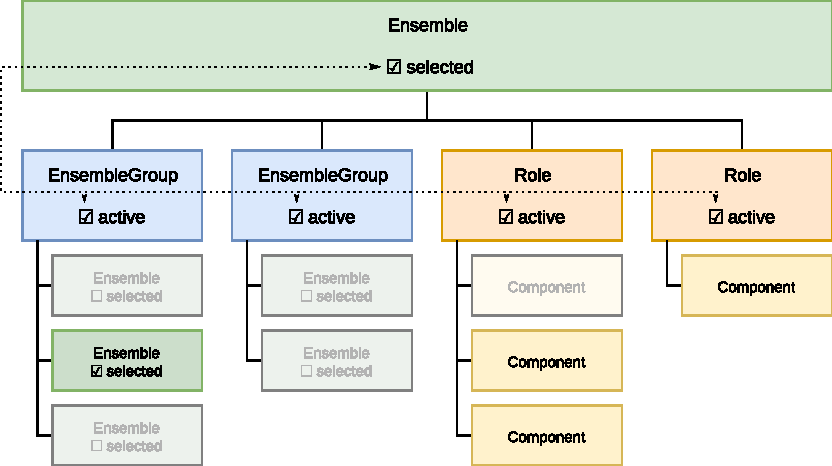
\includegraphics{img/classdia.pdf}
    \caption{Ensemble object diagram}
    \label{fig:objectdiagram}
\end{figure}

One notable feature is that an ensemble does not hold its members directly. Instead, it
holds \cc{MemberGroup}s. Selection parameters in each group are independent from other
groups; that way it is possible to have dynamically selected \cc{ensembles} and
selection enforcement by \cc{rules} in the same ensemble.

Ensembles also keep track of their own selection status. If an ensemble is selected in
its parent group, it can select its own members; more precisely, its groups are allowed
to select their members.

To facilitate this, ensemble has an \cc{isSelectedVar: BoolVar} representing the
selection status. When adding a role or an ensemble group, its \cc{isActiveVar} is set
to equal the parent ensemble's \cc{isSelectedVar}, as indicated on
figure~\ref{fig:objectdiagram} by the dotted line. If an ensemble is selected, all its
groups become active and can select members. If it is not selected, its groups are
inactive and the whole branch of the hierarchy is effectively turned off.

If an ensemble is part of an ensemble group, its \cc{isSelectedVar} is reified with the
corresponding membership constraint in the group's \cc{allMembersVar} (plus the result
of its situation predicate). The root ensemble is not a member of any groups, so its
\cc{isSelectedVar} is bound to true by the policy object.
